%%%%%%%%%%%%%%%%%%%%%%%%%%%%%%%%%%%%%%%%%%%%%%%%%%%%%%%%%%%%%%
%% LaTeX template for the science justification to be       %%
%%       submitted as part of an ALMA proposal.             %%
%%                                                          %%
%%                      ALMA Cycle 2                        %%
%%                                                          %%
%%%%%%%%%%%%%%%%%%%%%%%%%%%%%%%%%%%%%%%%%%%%%%%%%%%%%%%%%%%%%%

\documentclass[11pt, a4paper, onecolumn]{article}

\usepackage{graphics,graphicx}

% Load commands

\newcommand{\HRule}{\rule{\linewidth}{0.5mm}}
\newcommand{\Hrule}{\rule{\linewidth}{0.3mm}}
\newcommand{\ergseccm}{erg\,s$^{-1}$\,cm$^{-2}$}
\newcommand{\etal}{et\,al.}
\newcommand{\halpha}{H$\alpha$}
\newcommand{\lya}{Ly$\alpha$}
\newcommand{\lsim}{\raise0.3ex\hbox{$<$}\kern-0.75em{\lower0.65ex\hbox{$\sim$}}}
\newcommand{\mjpbeam}{\,\,mJy\,beam$^{-1}$}
\newcommand{\msun}{M$_{\odot}$}

% column densities
\newcommand{\hii}{H\,{\sc ii}}
\newcommand{\hi}{{\rm H\,{\sc i}}}
\newcommand{\nhi}{{$N$(\rm H\,{\sc i})}}
\newcommand{\hiColDens}{{$N($\rm H$_{\rm 2})$}}
\newcommand{\htwo}{{\rm H$_{\rm 2}$}}
\newcommand{\htwoColDens}{{$N($\rm H$_{\rm 2})$}}
\newcommand{\hisd}{$\Sigma_{\rm H\,{\text{\sc i}}}$}
\newcommand{\htwosd}{$\Sigma_{\rm H2}$}
\newcommand{\hsd}{$\Sigma_{\rm H}$}


\newcommand{\ii}{{\sc ii}}
\newcommand{\iii}{{\sc iii}}

% Units
\newcommand{\kms}{km\,s$^{-1}$}
\newcommand{\pom}{\,$\pm$\,}
\newcommand{\mm}{$\mu$m}
\newcommand{\lcdm}{$\Lambda$CDM}
\newcommand{\cm}{cm$^{-2}$}
\newcommand{\colDens}{$\times\ 10^{20}$ cm$^{-2}$}

% Units
\newcommand{\vrot}{$v_{\rm rot}$}
\newcommand{\vdisp}{$\sigma_{\rm HI}$}
\newcommand{\tspin}{$T_{\rm s}$}
\newcommand{\tdust}{$T_{\rm d}$}



% load packages
% Packages

% \usepackage{fancyhdr} % Required for custom headers
% \usepackage{lastpage} % Required to determine the last page for the footer
% \usepackage{extramarks} % Required for headers and footers
% \usepackage[usenames,dvipsnames]{color} % Required for custom colors
\usepackage{graphicx} % Required to insert images
% \usepackage{listings} % Required for insertion of code
% \usepackage{courier} % Required for the courier font
% \usepackage{dsfont} % For special math characters
% \usepackage{verbatim}

%\usepackage{amsmath, amssymb, bm} % For matrix notation
\usepackage[english]{babel}
\usepackage[paperwidth=8.5in,paperheight=11in,margin=1.0in]{geometry}
\usepackage{listings}
\usepackage{hyperref}
%\usepackage[cmex10]{amsmath, bm}
\usepackage{amsmath, bm}
\usepackage{blkarray}








% load formatting
\pdfcompresslevel0

% ==============================================================================
% PYTHON
% ==============================================================================
\usepackage[utf8]{inputenc}

% Default fixed font does not support bold face
\DeclareFixedFont{\ttb}{T1}{txtt}{bx}{n}{12} % for bold
\DeclareFixedFont{\ttm}{T1}{txtt}{m}{n}{12}  % for normal

% Custom colors
\usepackage{color}
\definecolor{deepblue}{rgb}{0,0,0.5}
\definecolor{deepred}{rgb}{0.6,0,0}
\definecolor{deepgreen}{rgb}{0,0.5,0}

\usepackage{listings}

% Python style for highlighting
\newcommand\pythonstyle{\lstset{
language=Python,
basicstyle=\ttm,
otherkeywords={self},             % Add keywords here
keywordstyle=\ttb\color{deepblue},
emph={MyClass,__init__},          % Custom highlighting
emphstyle=\ttb\color{deepred},    % Custom highlighting style
stringstyle=\color{deepgreen},
frame=tb,                         % Any extra options here
showstringspaces=false,            % 
breaklines=true
}}


% Python environment
\lstnewenvironment{python}[1][]
{\pythonstyle\lstset{#1}
}
{}

% Python for external files
\newcommand\pythonexternal[2][]{{
\pythonstyle\lstinputlisting[#1]{#2}}}

% Python for inline
\newcommand\pythoninline[1]{{\pythonstyle\lstinline!#1!}}
% ==============================================================================
% ==============================================================================

% Margins
\topmargin=-0.45in
\evensidemargin=0in
\oddsidemargin=0in
\textwidth=6.5in
\textheight=9.0in
\headsep=0.25in

\linespread{1.1} % Line spacing

% Set up the header and footer
\pagestyle{fancy}
\lhead{\hmwkAuthorName} % Top left header
\chead{\hmwkClass\ (\hmwkClassInstructor\ \hmwkClassTime): \hmwkTitle} % Top center head
\rhead{\firstxmark} % Top right header
\lfoot{\lastxmark} % Bottom left footer
\cfoot{} % Bottom center footer
\rfoot{Page\ \thepage\ of\ \protect\pageref{LastPage}} % Bottom right footer
\renewcommand\headrulewidth{0.4pt} % Size of the header rule
\renewcommand\footrulewidth{0.4pt} % Size of the footer rule

\setlength\parindent{0pt} % Removes all indentation from paragraphs

%----------------------------------------------------------------------------------------
%	DOCUMENT STRUCTURE COMMANDS
%	Skip this unless you know what you're doing
%----------------------------------------------------------------------------------------

% Header and footer for when a page split occurs within a problem environment
\newcommand{\enterProblemHeader}[1]{\nobreak\extramarks{#1}{#1 continued on next page\ldots}\nobreak\nobreak\extramarks{#1 (continued)}{#1 continued on next page\ldots}\nobreak}

% Header and footer for when a page split occurs between problem environments
\newcommand{\exitProblemHeader}[1]{\nobreak\extramarks{#1 (continued)}{#1 continued on next page\ldots}\nobreak\nobreak\extramarks{#1}{}\nobreak}

\setcounter{secnumdepth}{0} % Removes default section numbers
\newcounter{homeworkProblemCounter} % Creates a counter to keep track of the number of problems

\newcommand{\homeworkProblemName}{}
\newenvironment{homeworkProblem}[1][Problem \arabic{homeworkProblemCounter}]{ % Makes a new environment called homeworkProblem which takes 1 argument (custom name) but the default is "Problem #"
\stepcounter{homeworkProblemCounter} % Increase counter for number of problems
\renewcommand{\homeworkProblemName}{#1} % Assign \homeworkProblemName the name of the problem
\section{\homeworkProblemName} % Make a section in the document with the custom problem count
\enterProblemHeader{\homeworkProblemName} % Header and footer within the environment
}{\exitProblemHeader{\homeworkProblemName} % Header and footer after the environment
}

% Defines the problem answer command with the content as the only argument
\newcommand{\problemAnswer}[1]{\noindent\framebox[\columnwidth, resolution=600][c]{\begin{minipage}{0.98\columnwidth, resolution=600}#1\end{minipage}}}
% Makes the box around the problem answer and puts the content inside }

\newcommand{\homeworkSectionName}{}
\newenvironment{homeworkSection}[1]{ % New environment for sections within homework problems, takes 1 argument - the name of the section
\renewcommand{\homeworkSectionName}{#1} % Assign \homeworkSectionName to the name of the section from the environment argument
\subsection{\homeworkSectionName} % Make a subsection with the custom name of the subsection
\enterProblemHeader{\homeworkProblemName\ [\homeworkSectionName]} % Header and footer within the environment
}{
\enterProblemHeader{\homeworkProblemName} % Header and footer after the environment
}



%%%%%%%%%%%%%%%%%%%%%%%%%%%%%
%%%%% Start of document %%%%% 
%%%%%%%%%%%%%%%%%%%%%%%%%%%%%

\begin{document}
\pagestyle{plain}
\pagenumbering{arabic}
 
%%%%%%%%%%%%%%%%%%%%%%%%%%%%%
%%%%%% Title of proposal %%%%%
%%%%%%%%%%%%%%%%%%%%%%%%%%%%%

\begin{center} {\LARGE{\bf
%%
%% ENTER TITLE OF PROPOSAL BELOW THIS LINE
{Are Metallicity Gradients of Disks Affected by their Dark Matter Halos?}
%%
%%
}} \end{center} \bigskip

% PI
\centerline{\bf PI:\@
{Proposal ID 7}$^1$}

% Affiliation
\smallskip
$^1$University of Wisconsin Madison, USA
\smallskip

%-------------------------------------------------------------------------------
\section{Abstract}\label{sec:abstract}
%-------------------------------------------------------------------------------

    MaNGA's sample of 10,000 galaxies up to a redshift of 0.2 opens the doors
    to understanding the origin of metallicity gradients in disk galaxies.
    Hydrodynamical simulations show that both star formation rates changing
    with the radius and gas infall rates variable with radius are both viable
    origins of metallicity gradients in disks. We aim to test the latter
    hypothesis by investigating how the metallicity gradients change with dark
    matter distributions in galaxy disks.  The methods developed by the CALIFA
    collaboration \citep{sanchez14} will guide our derivation of the
    metallicities for a large sample of galaxies.   

    Our investigation using the MaNGA survey will consist of first deriving the
    gas-phase metallicity gradients using the O\iii\,$\lambda$5007, H$\beta$,
    N\ii\,$\lambda$6584, and H$\alpha$ lines.  We will derive detailed
    dark-matter distributions as a function of radius with the high-resolution
    kinematic and spatial resolution provided by MaNGA. We will compare star
    formation rates, gas distributions, and stellar mass distributions among
    the sample galaxies.
    
\begin{multicols}{2}
%-------------------------------------------------------------------------------
\section{Scientific Justification}
%-------------------------------------------------------------------------------

    Metals are fundamental to cooling mechanisms in the intergalactic and
    interstellar medium, star formation, stellar physics, and planet
    formation.  MaNGA will break new ground in understanding the chemical
    evolution of disk galaxies through observations of metallicity gradients.
    Metallicity gradients of disks have been studied heavily in smaller samples
    \citet{sanchez14} and on an individual basis, however, with MaNGA's sample
    of 10,000 galaxies we are presented a unique opportunity to understand
    metallicity gradients across a wide range of galaxy characteristics.

%-------------------------------------------------------------------------------
\subsection{The CALIFA Survey Results}
%-------------------------------------------------------------------------------

    A recent survey of $\sim$\,600 galaxies in the nearby universe, Calar Alto
    Legacy Integral Field Area Survey (CALIFA) \citep{sanchez12} provided
    nearly 7,000 \hii\ regions in $\sim$\,300 galaxies. \citet{sanchez14}
    derived gas-phase metallicities using the strong-line method finding that
    all galaxies without evidence of a merger have a common oxygen abundance
    gradient. See Figure~\ref{fig:sanchez} showing the common gradient. However
    CALIFA is a sample of 600 galaxies with redshifts 0.005 $< z <$ 0.03. MaNGA
    is a sample of 10,000 galaxies out to redshifts measured in the first data
    release of the Sloan Digital Sky Survey, $z \sim\,0.2$
    \citep{abazajian03}.  Metallicity gradients may evolve over time, and with
    MaNGA's larger sample-size we will be able to build off of the results of
    \citet{sanchez14} to test what factors affect the metallicity gradients in
    disks.

    %-----------------------------Figure Start---------------------------
    %\end{multicols}
    \begin{figure*}[!ht]

        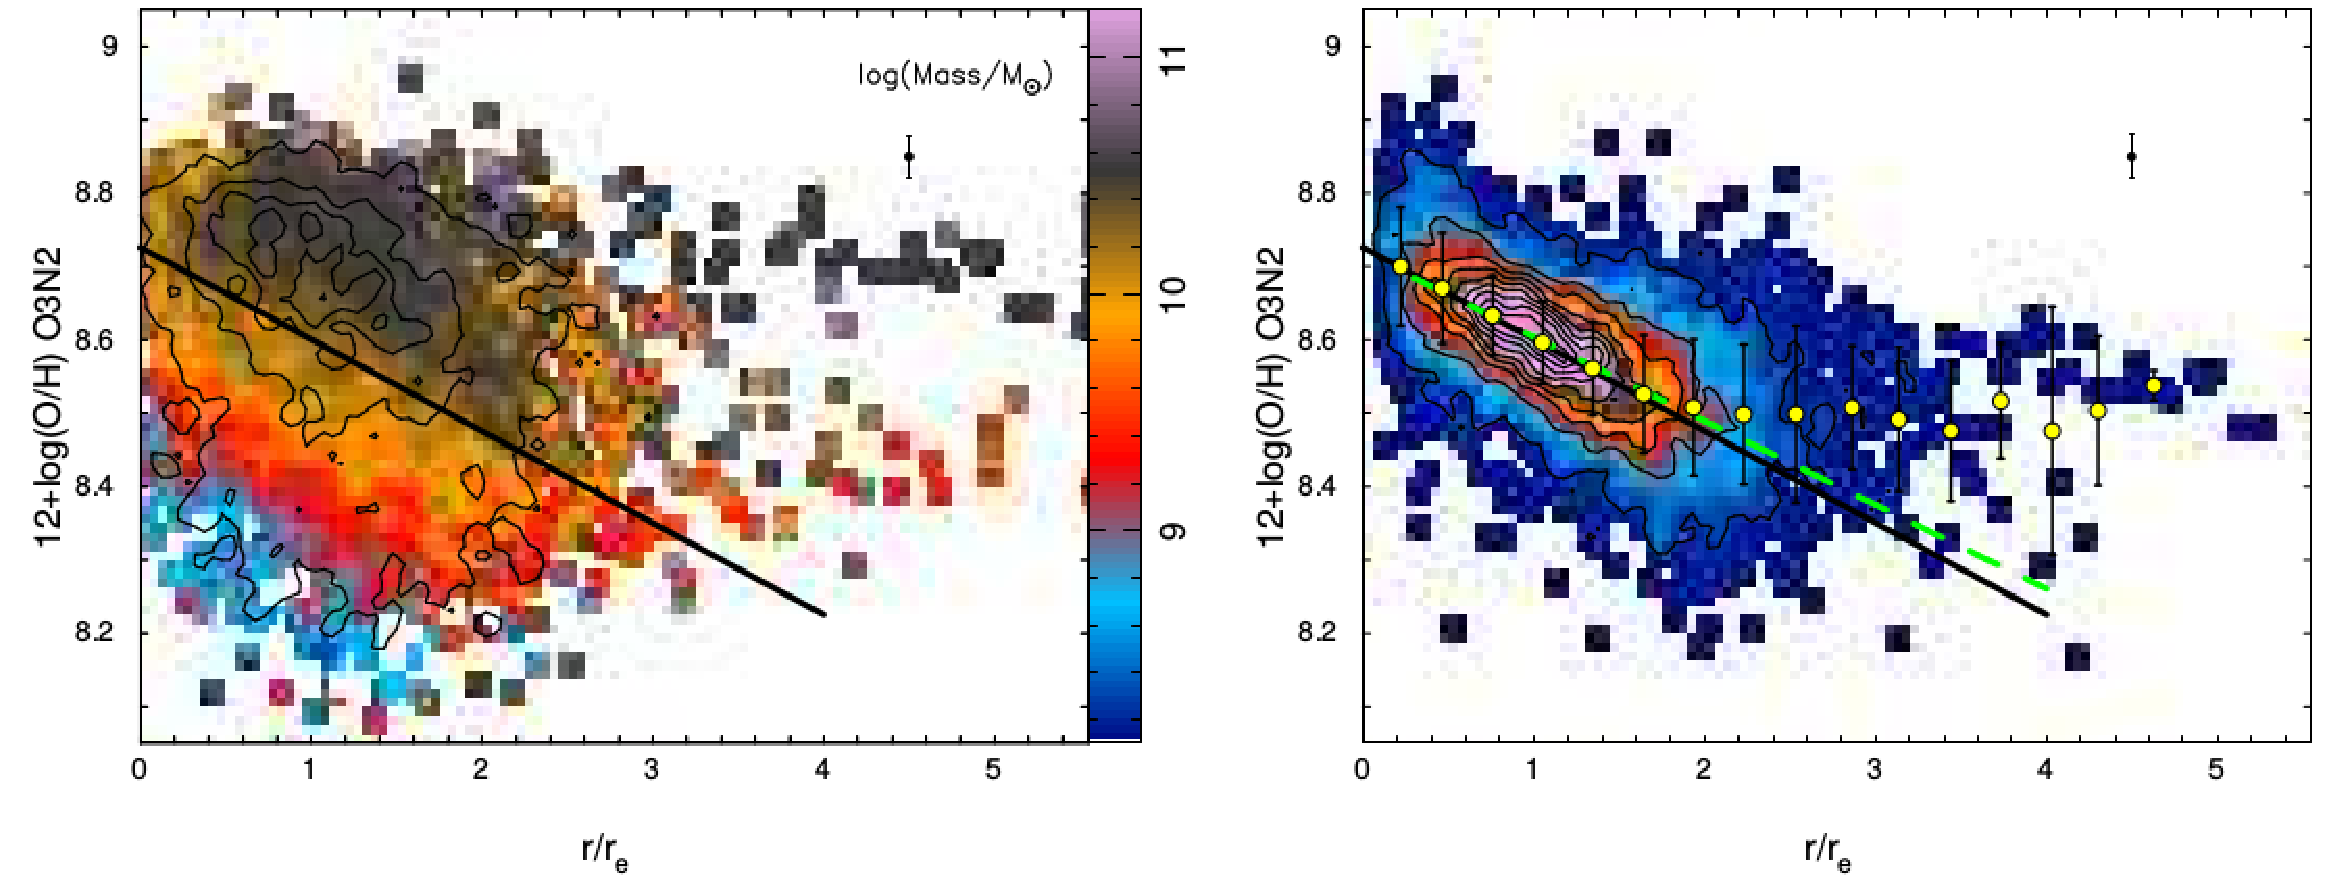
\includegraphics[scale=0.45]{figures/sanchez12_fig9.pdf}

        \caption{\label{fig:sanchez} Results from the CALIFA survey.
            \textit{Left panel:} Radial distribution for the oxygen abundance
            derived using the [O\iii] / [N\ii] indicator for all the galaxies
            in the CALIFA sample.  The contours show the density distribution
            of \hii\ regions. The outermost contour encircles 95\% of the total
            number of \hii\ regions, with $\sim$\,20\% less in each consecutive
            contour. The color bar shows the average stellar mass at the galaxy
            radius. This trend is indicative of the mass/metallicity
            relationship \citep{tremonti04}. \textit{Right panel:} Radial
            distribution for the oxygen abundance after scaling to the average
            value at the disk effective radius for each galaxy. The image and
            contours show the density distribution of \hii\ regions. The
            outermost contour encircles 95\% of the total of \hii regions, with
            $\sim$\,20\% less in each consecutive contour.  The solid-yellow
            points represent the average oxygen abundances. The solid-black
            lines in both panels represent the linear relation corresponding to
            the mean values of the zero-points and slopes of the individual
            regression derived for distributions of each individual galaxy. The
            dashed-green line shows the result of the best linear regression to
            the data. The characteristic slope derived is -0.1 dex/$r_e$
            between 0.3 and 2 disk effective radii ($r_e$). These results
            demonstrate that gas-phase metallicity gradients are both
            ubiquitous and significant in nearby galaxies.  Figure from
        \citet{sanchez14}.\/}

    \end{figure*}
    %\begin{multicols}{2}
    %-----------------------------Figure End------------------------------


%-------------------------------------------------------------------------------
\subsection{Creating Abundance Gradients}
%-------------------------------------------------------------------------------

    According to \citet{goetz92}, there are only 4 possible ways to create a
    radial abundance gradient: (1) A radial variation of the initial mass
    function (IMF); (2) A variation of the stellar yields with galactocentric
    radius; (3) A star formation rate (SFR) changing with the radius; (4) A gas
    infall rate variable with radius. No evidence exists for radial variations
    in the IMF, and radially-dependent stellar yields are already included in
    modern models, which adopt metallicity dependent stellar yields. Most
    chemical evolution models explain the gradients in gas-phase metallicity
    from the combined effects of a star formation rate and an infall of gas,
    both varying with galactocentric radius of galaxies.  \citet{gibson13} show
    with hydrodynamical simulations that the radial gradients are dependent on
    the feedback, star formation, and infall in galaxies. Thus we adopt the
    question: how do dark matter distributions affect the feedback, star
    formation and infall in galaxies?

%-------------------------------------------------------------------------------
\subsection{Dark Matter Distributions}
%-------------------------------------------------------------------------------

    Recent studies have shown that the dark matter halo profile in galaxies may
    in fact be affected by baryonic processes. \citet{dicintio14} found a clear
    dependence of the inner slope of the dark matter density profile on the
    stellar-to-halo mass ratio in their hydrodynamic simulations. At higher
    star formation efficiencies dark matter profiles become flatter.
    \citet{dicintio14b} introduced a mass-dependent density profile to describe
    the distribution of dark matter within galaxies, which takes into account
    the stellar-to-halo mass dependence of the response of dark matter to
    baryonic processes. When the ratio of the stellar mass to the halo mass is
    low, $\lesssim$\,0.01\%, energy from stellar feedback is insufficient to
    significantly alter the inner dark matter density, and the galaxy retains a
    cuspy profile. At higher stellar-to-halo mass ratios, feedback drives the
    expansion of the dark matter and generates cored profiles.
    \citet{teyssier13} found similar simulation results, showing that it is
    possible to form a prominent dark matter core within the well-controlled
    framework of an isolated, initially cuspy, 10$^{10}$ \msun\ dark matter
    halo using feedback mechanisms.

    Are feedback processes and the stellar masses which govern the shape of
    dark matter profiles the dominant cause of metallicity gradients, or do the
    altered dark matter profiles change the metallicity gradient themselves?

%-------------------------------------------------------------------------------
\subsection{Connecting Dark Matter to Metallicity Gradients}
%-------------------------------------------------------------------------------

    More evidence is growing that large-scale galactic outflows are the
    dominant cause of gas-phase metallicity gradients
    \citet{martel13,jones13}.  \citet{fu13} simulated disk galaxy evolution,
    finding that radial gas inflow has little influence on gas-phase and
    stellar metallicity gradients, which are affected much more strongly by the
    fraction of metals that are directly injected into the halo gas, rather
    than mixed with the cold gas.  Metals ejected out of the galaxy in early
    epochs result in late infall of pre-enriched gas and flatter present-day
    gas-phase metallicity gradients.  For galaxies with bulges, i.e. galaxies
    with recent mergers, the metallicity gradient is shallower due to newly
    accreted gas (See Figure~\ref{fig:fu}). \citet{spavone10} found that cold
    gas accretion is the most likely cause of the metallicity gradient in
    NGC\,4650A, whereby the dark matter profile could play a role in the manner
    in which the gas was accreted. How the gas flows back onto the disk of a
    galaxy will affect the metallicity gradient.
    
    %-----------------------------Figure Start---------------------------
    %\end{multicols}
    \begin{figure*}[!ht]

        \centering

        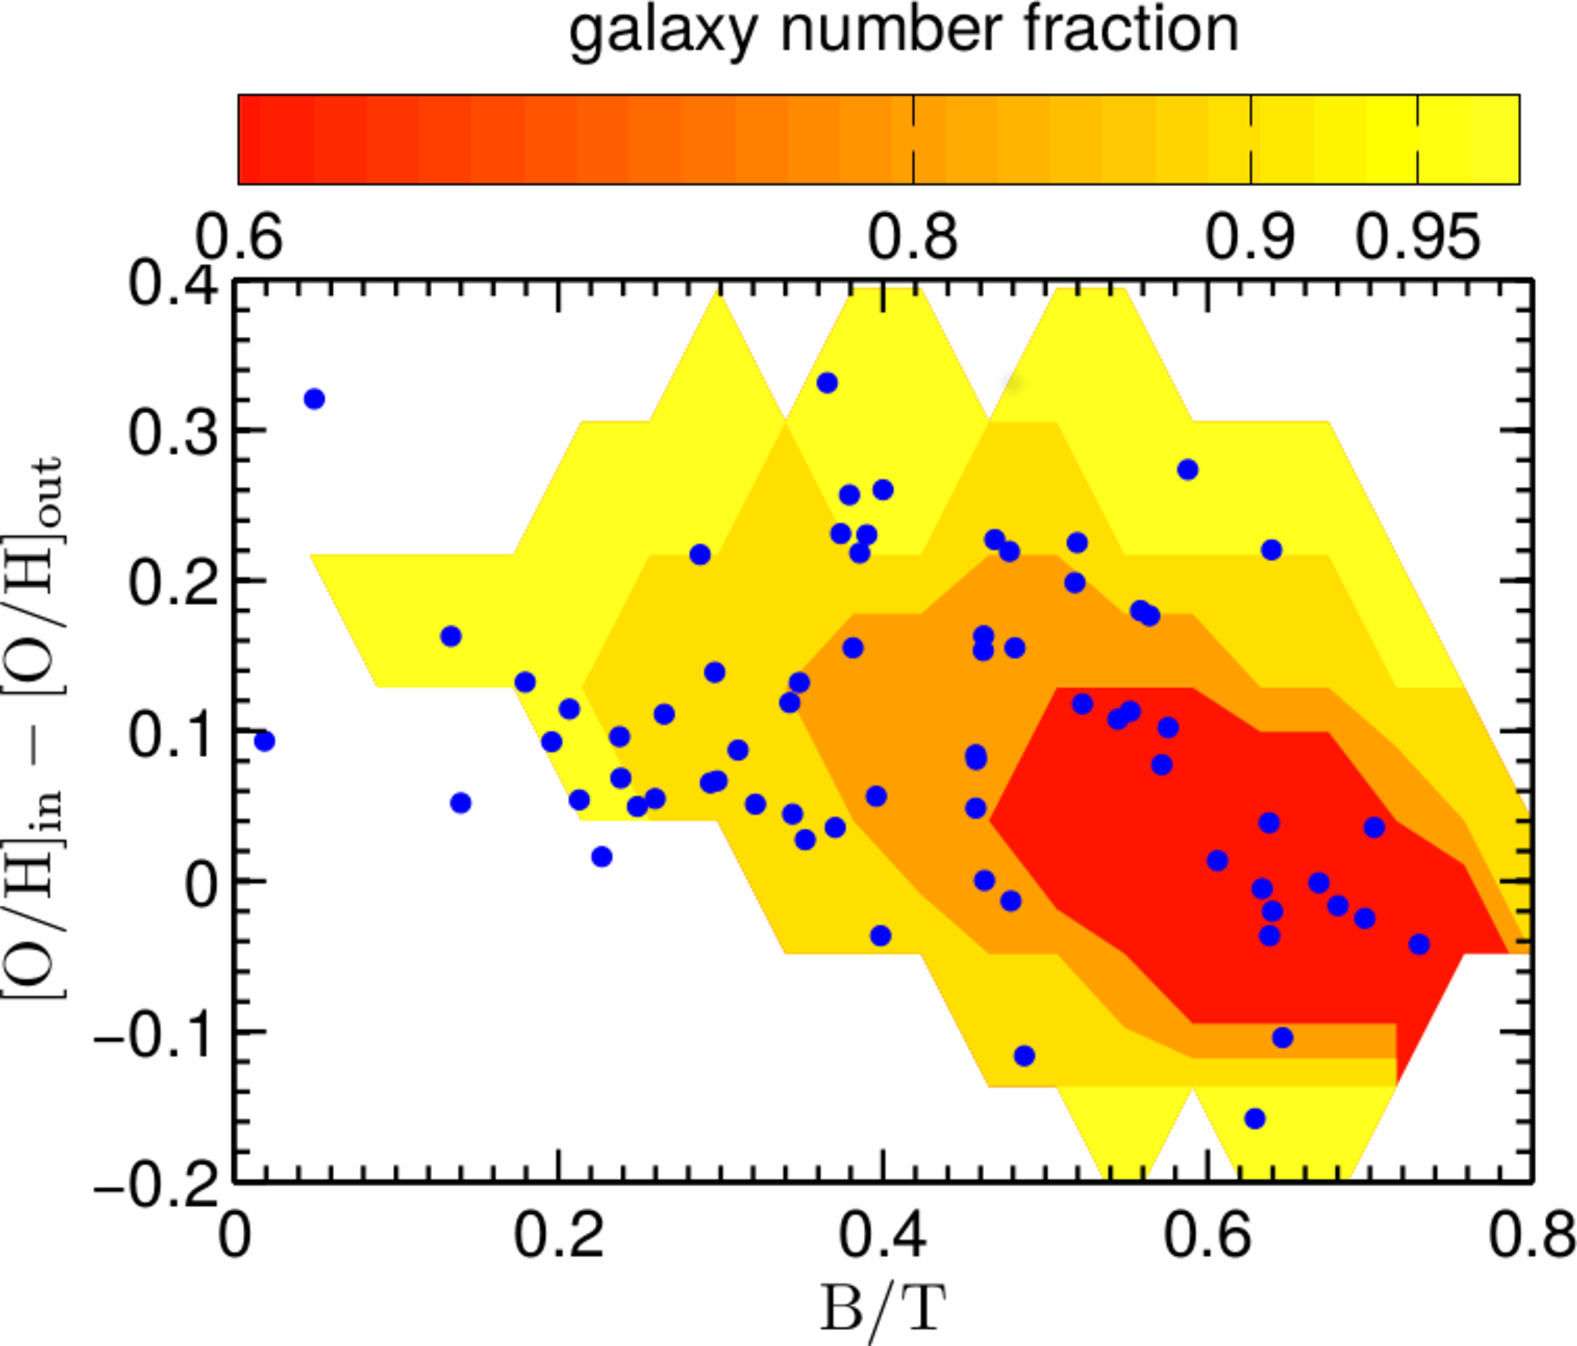
\includegraphics[scale=0.4]{figures/fu13_fig12.pdf}

        \caption{\label{fig:fu} Plotted is the oxygen abundance of the outer
            regions [O/H]$_{\rm out}$ of disks subtracted from the oxygen
            abundance of the inner regions [O/H]$_{\rm in}$ as a function of
            the bulge-to-total (B/T) galaxy mass. The blue dots are from
            \citet{moran12} data, obtained with long-slit spectra of 174
            star-forming galaxies with stellar masses greater than 10$^{10}$
            \msun\ from the GALEX Arecibo Sloan Digital Sky Survey survey. The
            contours indicate the fraction of model galaxies located in a given
            region of parameter space, as given by the color key at the top of
            the plot. We can see that steeper oxygen abundance gradients exist
            in disks with smaller bulge-to-total galaxy masses.  This is
            because gas is consumed when the bulge forms during galaxy mergers,
            and the gas-phase metallicity gradient is then set by
        newly-accreted gas. Figure from \citet{fu13}.\/}

    \end{figure*}
    %\begin{multicols}{2}
    %-----------------------------Figure End------------------------------

    Dark matter distributions are strongly coupled with the bar strengths and
    gas accretion. Infalling gas will distribute angular momentum into
    disks, but dynamical friction from the dark matter halo and bulge will
    cause the gas to fall towards the centers. When the dark mass inside the
    bar region is negligible, bars develop through angular momentum exchange
    between the inner and outer disk, and between stars and gas. During galaxy
    formation, baryons can lose most of their angular momentum if the infall of
    gas is misaligned with the dark matter axes \citep{combes13}. The flow of
    enriched gas back onto the disk will depend on the dark matter
    distribution, the bulge mass, and the presence of a bar.

    \begin{comment}
    \citet{jones13}  find that metallicity gradients and their evolution can be
    explained by the inward radial migration of gas together with a radial
    variation in the mass loading factor governing the ratio of outflowing gas
    to the local star formation rate. Metallicity gradients are caused by
    radial variation in the effective mass loading factor.

    \citet{portinari10} found by investigating rotation curves in the framework
    of variable mass-to-light ratio of stellar discs, they confirm the scenario
    obtained with the constant M$_*$/L assumption: a dark matter halo with a
    shallow core, an inner baryon-dominated region.

    \citet{martizzi13} used cosmological simulations to show that active
    galactic nuclei (AGN) feedback on the gas distribution in clusters of
    galaxies can be important in determining the spatial distribution of stars
    and dark matter in the central regions of these systems 
    
    \citet{tissera13} investigate the chemical and kinematic properties of the
    diffuse stellar halos of six simulated Milky-Way-like galaxies from the
    Aquarius Project. The observed abundance gradients in the inner-halo
    regions are influenced by both the level of chemical enrichment and the
    relative contributions from each stellar subpopulation. Steeper abundance
    gradients in the inner-halo regions are related to contributions from the
    disc-heated and endo-debris stars, which tend to be found at lower binding
    energies than debris stars. 

    \citet{mott13} We compute the abundance gradients along the disc of the
    Milky Way by means of the two-infall model: in particular, the gradients of
    oxygen and iron and their temporal evolution. First, we explore the effects
    of several physical processes which influence the formation and evolution
    of abundance gradients. They are (i) the inside-out formation of the disc,
    (ii) a threshold in the gas density for star formation, (iii) a variable
    star formation efficiency along the disc, (iv) radial flows and their speed
    and (v) different total surface mass density (gas plus stars) distributions
    for the halo. 
    
    \end{comment}

%-------------------------------------------------------------------------------
\section{The Experiment}
%-------------------------------------------------------------------------------
    The BOSS spectrographs, each with a red and blue arm will enable
    simultaneous wavelength coverage from 3600\,\AA\ to 10,000\,\AA\ to probe
    sensitive lines to the abundances of heavier elements. Our investigation
    using the MaNGA survey will consist of first deriving the gas-phase
    metallicity gradients using the O\iii\,$\lambda$5007, H$\beta$,
    N\ii\,$\lambda$6584, and H$\alpha$ lines to derive the oxygen abundances.
    We will derive detailed dark-matter distributions as a function of radius
    with the high-resolution kinematic and spatial resolution provided by
    MaNGA. We will compare star formation rates, gas distributions, and stellar
    mass distributions in each of our sample galaxies.

%-------------------------------------------------------------------------------
\subsection{Determining Locations of \hii\ Regions }
%-------------------------------------------------------------------------------

    Determining the presence and locations of \hii\ regions in a sample of
    10,000 galaxies is a daunting task. We will adopt the methods pioneered by
    \citet{sanchez14}. To detect \hii\ regions we will first use automatic an
    routine which subtracts the underlying stellar population and returns
    information on the strongest emission lines using the code
    \textsc{HIIexplorer} \citep{sanchez12b}. The assumptions in this analysis
    are (a) \hii\ regions are peaky/isolated structures with a strong ionized
    gas emission, clearly above the continuum emission and the average ionized
    gas emission across the galaxy; (b) \hii\ regions have a typical physical
    size of about a hundred or a few hundreds of parsecs.

    Distinguishing between low-ionization sources, like weak active galactic
    nuclei (AGN)s, shocks and/or post-AGBs stars requires a careful analysis of
    line ratios sensitive to the individual environments. The most common
    diagnostic diagram in the literature for the optical regime is the one
    which makes use of easily-observable strong lines that are less affected by
    dust attenuation, i.e., [O\iii]/\,H$\beta$ vs. [N\ii]/H$\alpha$
    \citep{baldwin81}. See Figure~\ref{fig:sanchez_b} for an example of the
    diagnostic diagram. \citet{kewley01} and \citep{kauffmann03} provide the
    diagnostic curves needed for determining \hii\ regions, the first derived
    from photodissociation models, and the second from empirical derivations
    from the SDSS sample. We will use the code \texttt{FIT3D} developed by
    \citet{sanchez12} in stellar-subtracted spectra to derive intensity,
    dispersion, and velocity of the required spectral lines.
    
    %-----------------------------Figure Start---------------------------
    \begin{figure*}[!ht]

        \centering

        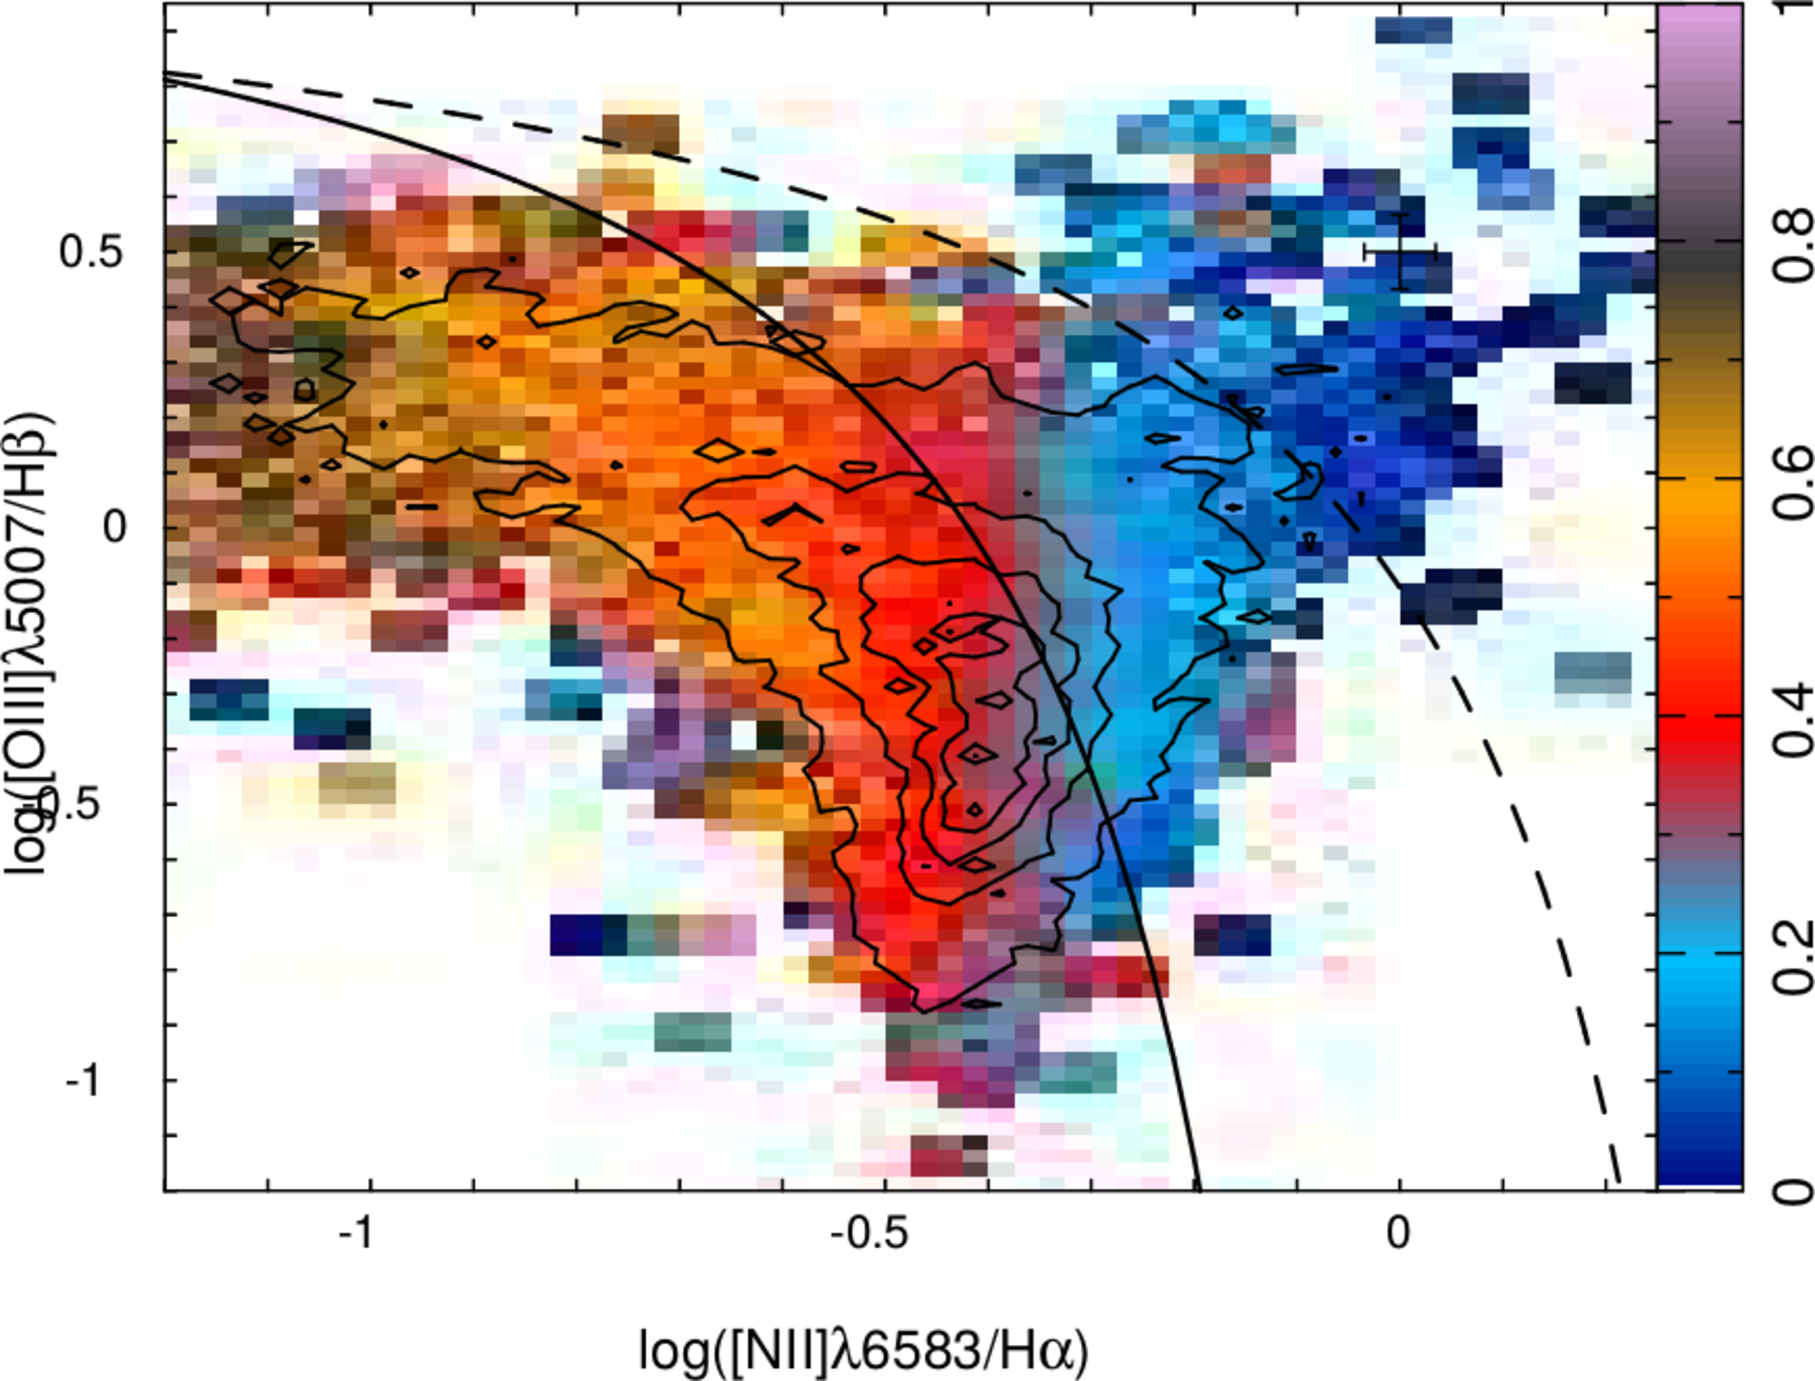
\includegraphics[scale=0.4]{figures/sanchez14_figure4.pdf}

        \caption{\label{fig:sanchez_b} [O\iii] $\lambda$5007/H$\beta$ vs.
            [N\ii] $\lambda$ 6583/H$\alpha$ diagnostic diagram for the
            $\sim$\,7,000 ionized regions described in the text. The contours
            show the density distribution of these regions with the diagram
            plane, with the outermost contour enclosing 95\% of the regions,
            and each consecutive one enclosing 20\% less regions. The color
            indicate the fraction of young stellar population in the underlying
            continuum. The solid- and dashed-line represent, respectively, the
            \citet{kauffmann03} demarcation curves. They are usually invoked to
            distinguish between classical star-forming objects (below the
            solid-line), and AGN powered sources (above the dashed-line).
            Regions between both lines are considered intermediate ones.  The
            higher concentration of young stellar populations below the
        solid-line provide confidence in the diagnostic tool, that \hii\
    regions from recent star formation consist of younger stellar populations.
Figure from \citet{sanchez14}.\/}

    \end{figure*}
    %-----------------------------Figure End------------------------------
    
%-------------------------------------------------------------------------------
\subsection{Oxygen Abundance Derivations}
%-------------------------------------------------------------------------------

    The next step will be to derive the gas-phase abundance of oxygen in the
    located \hii\ regions. We will use the ratio of \\
    
    \begin{math} \centering
        \frac{I(O\textsc{iii} \lambda5007) / I(H\beta)}
             {I(N\textsc{ii} \lambda6584) / I(H\alpha)}
    \end{math} \\

    to derive the oxygen abundance. \citet{stasinska06} derived empirical
    calibrations for this ratio which will provide us an accuracy of
    $\pm$\,0.08 dex of the oxygen abundance. MaNGA wide spectral coverage
    provides a unique opportunity to use the [O\iii] $\lambda$5007/[O\ii]
    $\lambda\lambda$3726,3729 ratio to solve for the ionization state, and
    thereby derive a more accurate oxygen abundance \citep{lopez-sanchez12}.
    MaNGA's low calibration errors of better than 2.4\% between H$\alpha$ and
    H$\beta$ will lend itself to robust derivations of the oxygen abundance.
    
    The H$\alpha$ line parameters will allow us to calculate the local star
    formation rate as a function of position using the calibration of
    \citep{kennicutt94}.

%-------------------------------------------------------------------------------
\subsection{Deriving Dark Matter Profiles}
%-------------------------------------------------------------------------------

    Our first steps will be to derive galaxy's initial mass function (IMF),
    because determining dark matter masses requires a-priori knowledge of the
    baryonic mass. \citet{conroy12} use a new population synthesis model that
    accounts for the effect of variable abundance ratios of 11 elements and
    analyze very high quality absorption line spectra of 38 early-type
    galaxies.  They are able to derive relationships between the [Mg/Fe] ratio
    and the IMF. With these state-of-the-art models we will be able to
    determine the baryonic contributions to a galaxy's mass.

    MaNGA offers a unique opportunity to have a uniform sample of kinematic and
    dynamical information for thousands of galaxies. The large spectral
    coverage of MaNGA offers a suite of spectral lines available for
    determining velocities as a function of position in the galaxy. With this
    information we will be able to follow the methods of \citet{cappellari13}
    who constructed detailed dynamical models (JAM), based on the Jeans
    equations and allowing for orbital anisotropy, for the volume-limited and
    mass-selected ATLAS$^{\rm 3D}$ sample of early-type galaxies
    \citep{cappellari11}. The models fit the two-dimensional galaxy images and
    reproduced in detail the integral-field stellar kinematics out to about 1
    projected half-light radius, $R_e$. They derived accurate total
    mass-to-light ratios and dark matter fractions with a sphere of radius $r =
    R_e$ centered on the galaxies.

    Additionally, for late-types we will adopt the methods of \citet{hague13}
    who employed a Markov Chain Monte Carlo approach to explore the parameter
    space of general dark matter profiles. They found that velocity errors are
    the most limiting factor in modeling, while spatial resolution is not. The
    model revealed the degeneracies between stellar and dark matter
    contributions for higher surface-brightness galaxies, thus we will be able
    to limit our derived sample of late-type galaxies to those with robustly
    calculated dark matter profiles. 
    
    MaNGA's median spatial resolution in the sample will be 1--2 kpc delivering
    unprecedented spatial resolution for a large sample of galaxies. The survey
    will provide the necessary chemical information for deriving IMFs, and the
    kinematic information at detailed spatial resolutions for dark matter
    profile modeling.

%-------------------------------------------------------------------------------
\subsection{Expected Results}
%-------------------------------------------------------------------------------

    We expect to derive dark matter distributions on kpc scales, with
    metallicity gradients on the same or larger scales. The results of
    \citet{dicintio14,dicintio14b} suggest that the galaxies with higher
    stellar-to-dark mass ratios will have more cored profiles, while galaxies
    with lower ratios will have more cuspy profiles. If gas inflow of ejected
    metal-rich gas during a previous epoch in star formation is the cause of
    metallicity gradients late- and early-types, then one would expect to see
    shallower gradients with more diffuse dark matter profiles hosted by
    galaxies with higher stellar-to-dark mass ratios. Dynamic friction between
    the dark matter halo and the infalling gas will cause the gas to fall into
    the disk. We will examine the relationships between the shapes of the
    dark-matter profiles and the metallicity gradients. We will also compare
    the star-formation rates of the galaxies in our sample with the metallicity
    gradients to investigate the other likely culprit in creating metallicity
    gradients.

%-------------------------------------------------------------------------------
\section{Summary}
%-------------------------------------------------------------------------------

    We propose to conduct an investigation with the MaNGA survey of how dark
    matter distributions affect the gas-phase oxygen abundance gradients in
    disk galaxies. Infall of previously ejected metal-rich gas is a viable
    origin for metallicity gradients in disks. How the gas falls back in to the
    disk will depend on the shape of the dark matter profile. Our analysis
    using the O\iii\ and N\ii\ indicators and detailed modeling of the stellar
    kinematics will allow for us to compare exactly how the dark matter
    distributions in galaxies affects the radial gas-phase oxygen abundance as
    a function of position in the galaxies. The MaNGA survey will allow us
    understand metallicity-halo profile relationships out to a redshifts of $z
    \sim 0.2$, potentially probing different epochs in gradient evolution.

    \bibliography{my_bib}
    
\end{multicols}

\end{document}

